\documentclass[tikz]{standalone}
\usepackage{tikz-3dplot}
\usepackage{graphicx}
\usepackage{amsmath}
\usepackage{mathspec}
\setromanfont[Numbers={Lining,Proportional}]{Minion Pro}
\setmathsfont(Digits,Latin,Greek)[Numbers={Lining,Proportional}]{Minion Pro}
\setmathrm{Minion Pro}
\usepackage{fix-cm}
\tdplotsetmaincoords{57}{43} %43,12
\newcommand{\ket}[1]{\left\lvert #1 \right\rangle}

\begin{document}
\begin{tikzpicture}[level/.style={thick}]
    \begin{scope}[scale=0.5,xshift=9cm,yshift=11.5cm]
        \pgftext{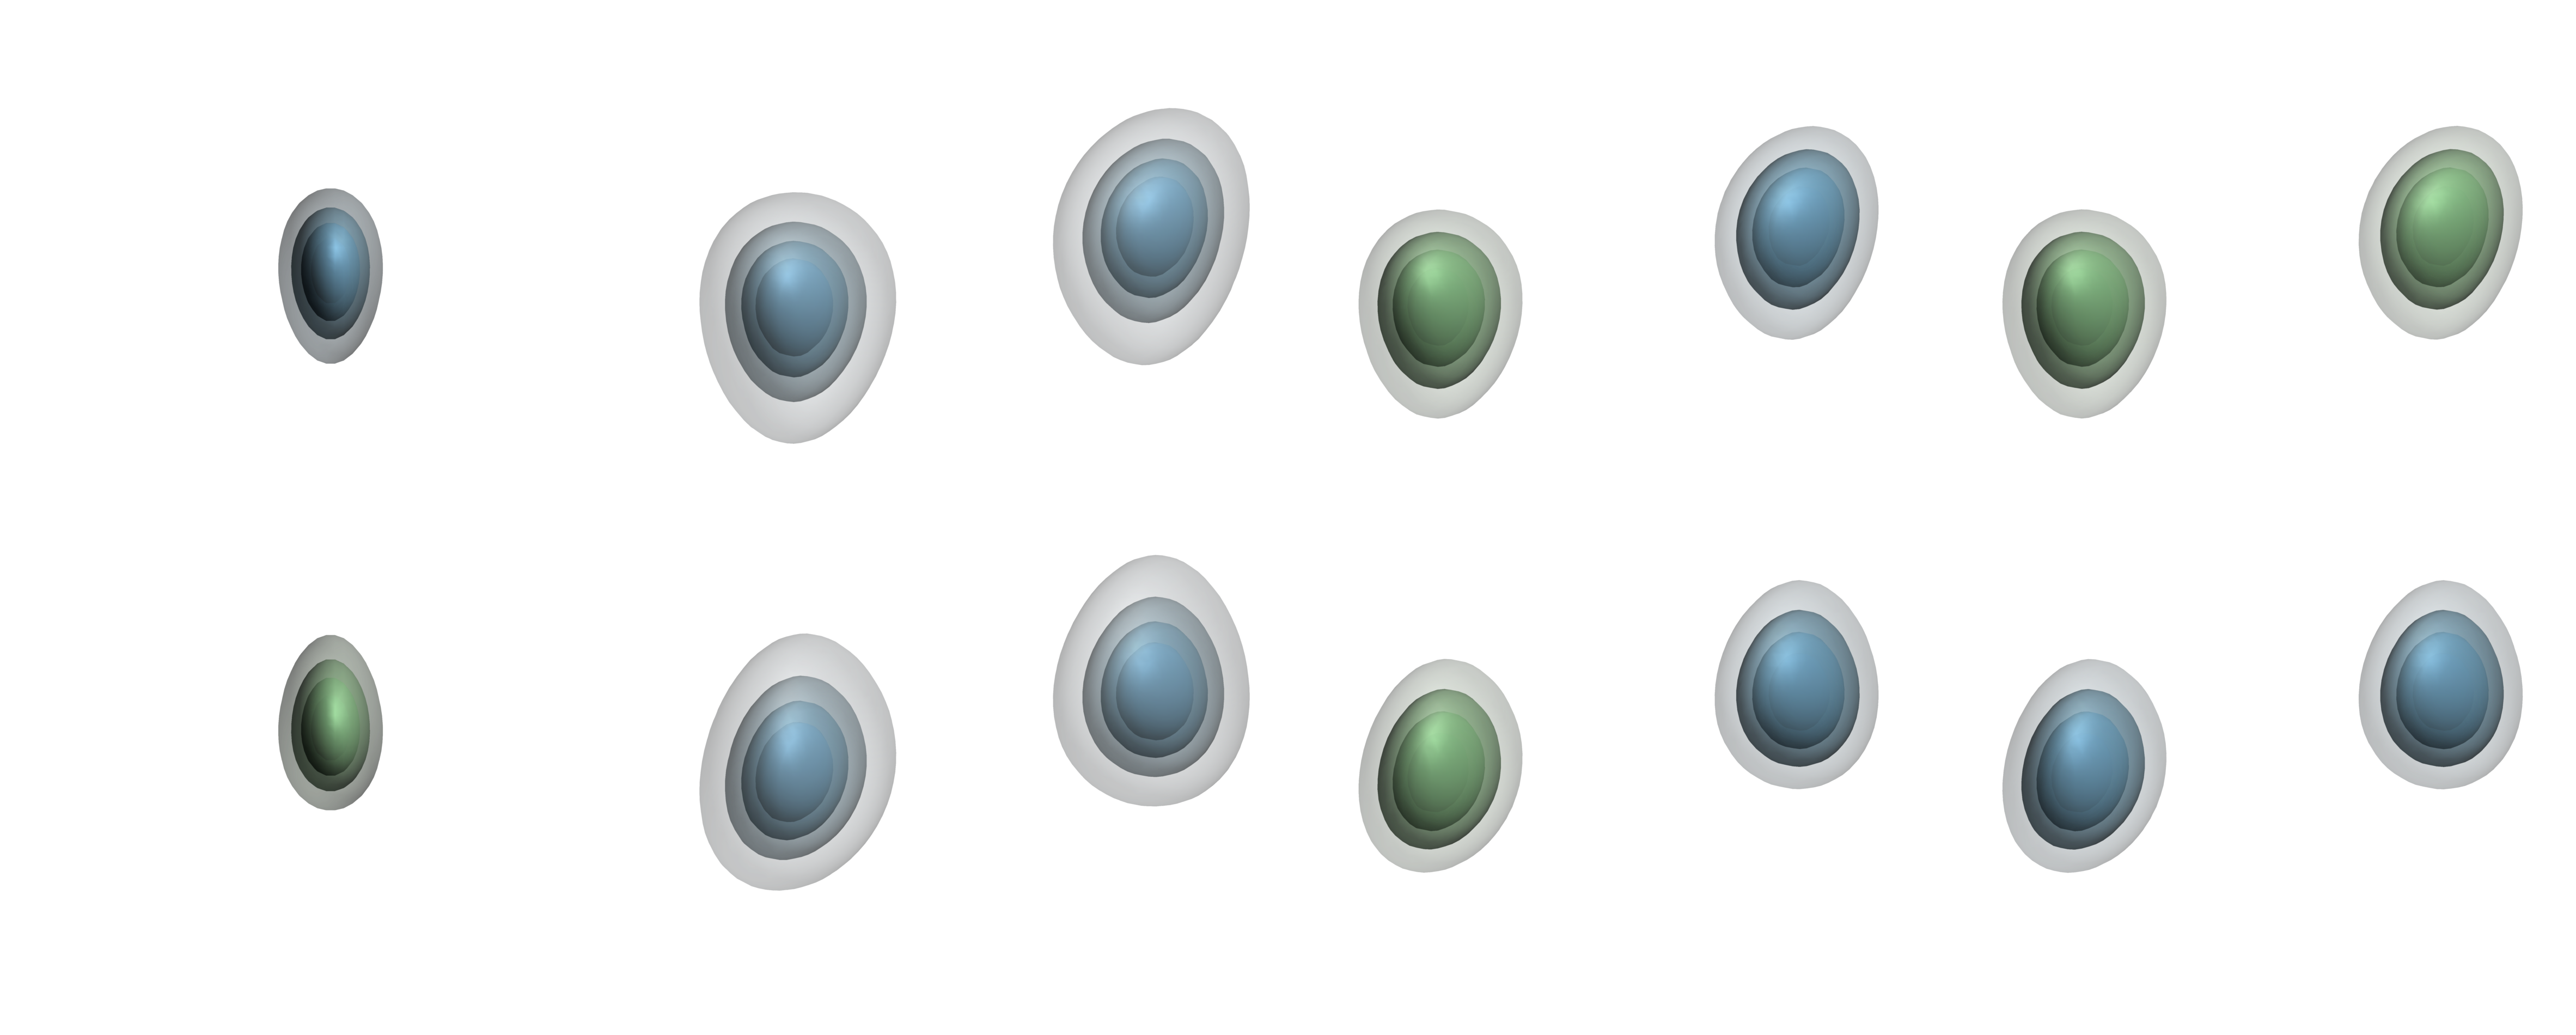
\includegraphics{atypey.png}};
    \end{scope}
 \begin{scope} [yshift=3.3cm,xshift=-0.15cm]
        \node (0,0) {\Large $\ket{1}$};
    \end{scope}
    \begin{scope} [yshift=3.3cm,xshift=3.1cm]
        \node (0,0) {\Large $\ket{0}$};
    \end{scope}
    \begin{scope} [yshift=3.3cm,xshift=6.2cm]
        \node (0,0) {\Large $\ket{1}$};
    \end{scope}
    \begin{scope} [yshift=3.3cm,xshift=9.3cm]
        \node (0,0) {\Large $\ket{2}$};
    \end{scope}
    \begin{scope}[yshift=4.1cm, xshift=-0.6cm]
        \draw[-stealth] (0,0,0) -- (1,0,0) node[below] {x};
        \draw[-stealth] (0,0,0) -- (0,3.5,0) node[right] {y};
    \end{scope}

    \begin{scope}[tdplot_main_coords, scale=1.5,yshift=0.5cm,xshift=1cm]
        \draw[-stealth] (0,0,0) -- (1,0,0) node[below] {x};
        \draw[-stealth] (0,0,0) -- (0,1,0) node[right] {y};
        \draw[-stealth] (0,0,0) -- (0,0,1) node[left] {z};
    \end{scope}
    
    \begin{scope}[yscale=0.5,xshift=4.5cm]
        \draw[level] (3,0) node[above=0.1em, right] {$E_{01} = 40.63$ MHz} -- (0,0) node[below=0.4em, left] {$E_{0}$};
        \draw[level] (3,0.2) node[above=2.4em, right] {$E_{12} = 1.14$ GHz} -- (0,0.2) node[above=0.4em, left] {$E_{1}$};
        \draw[level] (3,3.5) -- (0,3.5) node[left] {$E_{2}$};
    \end{scope}
\end{tikzpicture}
\end{document} 